%
% Monografia de TCC1 de Douglas Brauner
%
\documentclass[twoside,english,brazilian]{UNISINOSmonografia}
\usepackage[utf8]{inputenc} % charset do texto (utf8, latin1, etc.)
\usepackage[T1]{fontenc} % encoding da fonte (afeta a sep. de sílabas)
\usepackage{graphicx} % comandos para gráficos e inclusão de figuras
\usepackage{bibentry} % para inserir refs. bib. no meio do texto
\usepackage{tabularx}
%=======================================================================
\unisinosbst

%=======================================================================
% Dados gerais sobre o trabalho.
%=======================================================================
\autor{Brauner}{Douglas}
\titulo{Elasticidade Baseada em Containers para Aplicação de Alto Desempenho}
%\subtitulo{sub}
\orientador[Prof.~Dr.]{Righi}{Rodrigo da Rosa}
%\coorientador[Prof.~Dr.]{Lamport}{Leslie}
\local{São Leopoldo}
\ano{2016}

\unidade{Unidade Acadêmica Graduação}
\curso{Curso de Bacharelado em Ciência da Computação}
\natureza{%
Trabalho de Conclusão de Curso apresentado como requisito parcial
para a obtenção do título de Bacharel em Ciência da Computação
pela Universidade do Vale do Rio dos Sinos --- UNISINOS
}

% cada palavra-chave deve ser fornecida duas vezes, uma em português e
% outra no idioma estrangeiro (na verdade, em tantos idiomas quantos se
% desejar).
% Se não fizer isto, não compila!
% TODO: adicionar mais palavras-chave
\palavrachave{brazilian}{Computação em Nuvem}
\palavrachave{brazilian}{Elasticidade}
\palavrachave{brazilian}{Containerização}
\palavrachave{english}{Cloud Computing}
\palavrachave{english}{Elasticity}
\palavrachave{english}{Containerization}
%palavrachave{}


%=======================================================================
% Início do documento.
%=======================================================================
\begin{document}
\capa
\folhaderosto
%\folhadeaprovacao % não deve ser incluída nos TCCs

%=======================================================================
% Dedicatória (opcional).
%
% O texto é normalmente colocado na parte de baixo da página, alinhado
% à direita.  Mas a formatação é basicamente livre.  Só não se escreve
% a palavra 'dedicatória'.
%=======================================================================
\begin{dedicatoria}
Aos nossos pais.\\[4ex] % quebra a linha dando um espaçamento maior
\begin{itshape} % faz o texto ficar em itálico
If I have seen farther than others,\\
it is because I stood on the shoulders of giants.\\
\end{itshape}
--- \textsc{Sir Isaac Newton} % \textsc é o "small caps"
\end{dedicatoria}

%=======================================================================
% Agradecimentos (opcional).
%=======================================================================
\begin{agradecimentos}
Obrigado!
\end{agradecimentos}

%=======================================================================
% Epígrafe (opcional).
%
% ``[...] o autor apresenta uma citação, seguida de indicação de autoria,
% relacionada com a matéria tratada no corpo do trabalho. Podem, também,
% constar epígrafes nas folhas de aberturas das seções primárias.''
%=======================================================================
\begin{epigrafe}
``\textit{Ninguém abre um livro sem que aprenda alguma coisa}''.\\
(Anônimo)
\end{epigrafe}

%=======================================================================
% Resumo em Português.
%
% A recomendação é para 150 a 500 palavras.
%=======================================================================
\begin{abstract}
A definir
\end{abstract}


\begin{otherlanguage}{english}
\begin{abstract}
A definir
\end{abstract}
\end{otherlanguage}

%=======================================================================
% Lista de Figuras (opcional).
%=======================================================================
%\listoffigures

%=======================================================================
% Lista de Tabelas (opcional).
%=======================================================================
%\listoftables

%=======================================================================
% Lista de Abreviaturas (opcional).
%
% Deve ser passada como parâmetro a maior das abreviaturas utilizadas.
%=======================================================================
%\begin{listadeabreviaturas}{seg., segs.}
%\item[ampl.] ampliado, -a
%\item[atual.] atualizado, -a
%\item[coord.] coordenador
%\item[N.~T.] Novo Testamento
%\item[seg., segs.] seguinte, -s
%\end{listadeabreviaturas}

%=======================================================================
% Lista de Siglas (opcional).
%
% Deve ser passada como parâmetro a maior das siglas utilizadas.
%=======================================================================
%\begin{listadesiglas}{FAPERGS}
%\item[ABNT] Associação Brasileira de Normas Técnicas
%\item[CAPES] Coordenação de Aperfeiçoamento de Pessoal de Nível Superior
%\item[FAPERGS] Fundação de Amparo à Pesquisa do Estado do Rio Grande do Sul
%\end{listadesiglas}

%=======================================================================
% Lista de Símbolos (opcional).
%
% Deve ser passado o maior (mais largo) dos símbolos utilizados.
%=======================================================================
%\begin{listadesimbolos}{Ca}
%\item[\textsuperscript{o}C] Graus Celsius
%\item[Al] Alumínio
%\item[Ca] Cálcio
%\end{listadesimbolos}

%=======================================================================
% Sumário
%=======================================================================
\tableofcontents

%=======================================================================
% Introdução
%=======================================================================
\chapter{Introdução}

% as epígrafes nos capítulos são opcionais

%\epigrafecap{The reasonable man adapts himself to the world; the unreasonable one persists in trying to adapt the world to himself. Therefore all progress depends on the unreasonable man.}{George Bernard Shaw}

%Conforme \citetexto{Hexsel11}, a introdução tem o objetivo de ``\emph{introduzir} o material que vai ser apresentado em mais detalhe nas seções subseqüentes''. Na introdução você deve contextualizar o problema e mostrar por que vale a pena resolvê-lo. Você deve apresentar a solução proposta e mostrar o seu diferencial em relação aos trabalhos relacionados. Observe, porém, que na introdução você deve apenas tratar do O QUÊ e PORQUÊ, sem tratar do como \cite{Hexsel11}, que deve ser explicado na seção que descreve o trabalho desenvolvido.
A definir
\begin{itemize}
	\item \textbf{Contexto e motivação:} 

	\item \textbf{Problema:}Considerando o cenário atual de aplicações HPC iterativas, bem como a elasticidade que containers oferecem, o trabalho aqui disposto busca responder a seguinte questão:
	\textit{Como seria o modelo de elasticidade em nuvem adaptado para o uso de containers para aplicações HPC iterativas, que possa gerar um ganho significativo de economia de recursos?} 
	\item \textbf{Objetivos:} 
	\begin{itemize}
		\item Desenvolver um modelo de elasticidade automática adaptada para uso de containers, para aplicações de Computação de Alto Desempenho, em ambientes de computação em nuvem, com foco em otimizar a utilização de recursos, em comparação ao método de elasticidade automática baseado em virtualização de máquinas.  
	\end{itemize}
	\begin{itemize}
		\item Objetivo geral --- qual o propósito da pesquisa?
		\item Objetivos específicos --- abertura do objetivo geral em outros menores (possíveis capítulos).
	\end{itemize}
\end{itemize}

%=======================================================================
% Fundamentação Teórica
%=======================================================================
\chapter{Fundamentação Teórica}

\section{Computação em Nuvem}
Segundo a definição do National Institute of Standards and Technologies (NIST) \cite{Mell2012}, a computação em nuvem é um modelo que permite o acesso de recursos computacionais configuráveis e compartilhados, de forma conveniente, ubíqua e sob demanda, capazes de ser provisionados e entregues com baixo custo de gerenciamento e sem a intervenção de um provedor de serviços. Tais recursos podem ser: redes, servidores, serviços, armazenamento, aplicações, etc. Tais recursos são tipicamente fornecidos no modelo \textit{pay-as-you-go}, ou seja, você paga de acordo com a demanda de recursos solicitada \cite{Suleiman2012}. Sendo assim, a computação em nuvem se utiliza de mecanismos para escalar estes recursos conforme necessidade, através de algoritmos que irão trabalhar no balanceamento de carga rapidamente para diminuir o desperdício de recursos computacionais.
Algumas abordagens deixam o gerenciamento de balanceamento de carga e recursos por conta da aplicação, que se faz uso de API (\textit{Application Program Interface}) para definir por meio de codificação dentro da própria implementação o controle. Esta abordagen requer que a implementação tenha consciência dos pontos específicos de implementação do controle, o que pode fugir do foco principal do programa. Outras tecnologias oferecem um mecanismo externo à aplicação para o controle de recursos utilizados, deixando para a aplicação apenas determinar os pontos de chamada de sistema para reorganizações necessárias na topologia de comunicação. 


% TODO: Diferenciar elasticidade e escalabilidade
\section{Elasticidade vs Escalabilidade}

A escalabilidade de uma aplicação se diz respeito à quantidade de usuários que ela pode manter conectados ao mesmo tempo, sendo o limite de escalabidade o ponto em que esta não pode suportar mais usuários conectados sem apresentar a mesma  eficiência \cite{Wilder12}. Uma aplicação pode ter a sua escalabilidade estendida através do fornecimento de recursos de \textit{hardware} adicionais, como memória, CPU, largura de banda, etc. No contexto de uma aplicação HPC, uma escalabilidade não se detêm apenas ao número de usuários suportados, mas também ao tipo de processamento que a aplicação precisa executar e que pode precisar de recursos adicionais para continuar desempenhando de forma efetiva. 


\section{Virtualização vs Containerização}

Uma camada de virtualização pode ajudar a isolar um ambiente compartilhado de computadores. Em clusters de HPC, normalmente os recursos são compartilhados entre mais usuários e isto faz com que possa ocorrer problemas nesse compartilhamento \cite{Xavier2013}.
A camada de virtualização baseada em container possui uma performance muito superior à virtualização pura, segundo a pesquisa deles.



\subsection{Containers}

A palavra \textit{container} ficou popularizada a partir de uma técnica de isolamento de recursos dentro de um sistema operacional baseado em UNIX, desde a release do sistema operacional Solaris 10 em 2005. A ideia era não somente restringir o acesso de recursos dentro deste container, mas também permitir uma proteção de recursos explicitamente dedicados à estes containers. Embora seja considerada como uma \textit{best practice} em desenvolvimento, a utilização de containers é bastante complexa e o mal uso pode levar à criação de aplicações com brechas de segurança, embora se pressuponha o contrário, diferente da facilidade que se tem com a utilização de máquinas virtuais (VM). Uma das implementações atuais de containers é o Linux Containers (LXC), que provê uma série de ferramentas que trabalham nativamente em sistemas operacionais baseado em UNIX para fornecer um ambiente semelhante ao que se obtêm com VM's, mas sem a sobrecarga de rodar um kernel separado e fazer simulação de hardware, através de utilização de namespaces, e \textit{control groups} \cite{LXC2016}.
Recentemente, a utilização de containers se popularizou em meio ao desenvolvimento de computação para a nuvem por causa da nova ferramenta chamada \textit{Docker}, criada em 2013 e inicialmente baseada no LXC como um provedor de runtime. Segundo \cite{NICKOLOFF2016}, Docker é um conjunto de ferramentas e serviço que facilitam a criação e manipulação de containers dentro de um sistema baseado em UNIX. Com Docker, é possível ter todas as vantagens de utilização de containers, porém sem o alto custo de configuração e com containers fornecidos seguindo as melhores práticas. 

\subsection{cgroups}
Cgroups é uma configuração que faz parte do subsistema de kernel de sistemas baseado em UNIX, que fornece controle sobre recursos do sistema, como CPU, memória, rede, etc. O cgroups, ou control groups esta presente na implementação de containers de Docker e é utilizado como mecanismo base de gerenciamemnto de recursos \cite{NICKOLOFF2016}.

% Substituir o uso de VM no autoelastic e fazer testes de viabilidade de containers no lugar
% verificar vantagens e novas oportunidades que o autoelastic pode ter com containers.
% Fazer um comparativo - Docker vale a pena?
% Talvez modificar o formato de balanceamento de carga, já que containers podem ter menor custo.

\subsection{Docker}
O Docker, apesar de inicialmente utilizar o LXC como provedor de runtime, criou uma implementação própria de ferramenta para criação de containers, procurando resolver algumas limitações da implementação de LXC, como segurança e simplificação [ref]. 

\subsection{Virtualização baseada em Hypervisor}
Um \textit{hypervisor}, ou gerenciador de máquinas virtuais, é um programa que roda no sistema operacional host, fornecendo os recursos de hardware deste para uma série de máquinas virtuais, neste caso, estas máquinas virtuais compartilham o mesmo hardware. Como mostrado na figura~\ref{fig:vmvsdocker}, o hypervisor é responsável por fornecer o acesso aos recursos para cada sistema operacional dentro das máquinas virtuais, mas com o custo deste gerenciamento como processamento, já que a ferramenta procura fornecer comportamento fiel de hardware para as máquinas virtuais \cite{Zhang2016}.

\subsection{Virtualização baseada em container}

O termo \textit{containerização} é a forma popular para se referenciar à virtualização baseada em container, que permite o isolamento de determinados softwares, que são executados dentro do mesmo kernel no sistema operacional Linux, mas que diferentemente do hypervisor, não adiciona uma camada virtualização, na qual precisaria carregar um sistema operacional convidado \cite{Zhang2016}, como mostra a figura~\ref{fig:vmvsdocker}.
\cite{Dua2014}

\subsection{Figuras}
A Figura~\ref{fig:vmvsdocker} ilustra a diferença entre uma aplicação em uma camada de virtualização por Docker e VM.

\begin{figure}
	\caption{Docker vs Virtual Machine}
	\label{fig:vmvsdocker}
	\centering%
	\begin{minipage}{.8\textwidth}
		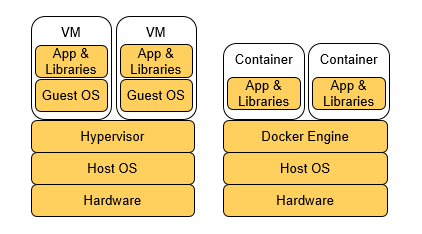
\includegraphics[width=\textwidth]{vmvsdocker}
		\fonte{\citetexto{Cham12}}
	\end{minipage}
\end{figure}

\begin{table}[!ht]
	\caption{Características de VM e Containers}
	\label{tab:table1}
	\centering%
	\begin{center}
		\begin{tabularx}{\textwidth}{|X|X|X|}
			\hline
			\textbf{Parametro} &\textbf{Máquinas Virtuais}\ &\textbf{Containers}\\
			\hline
			SO Convidado &Um hardware virtual é disponibilizado para cada VM, com um espaço de memória reservado. & Todos os convidados compartilham o mesmo SO, cada imagem é carregada para o espaço de memória do Kernel\\
			Comunicação & Feita por dispositivos Ethernet & Utilização de mecanismos IPC como sinais, sockets, pipes\\
			Segurança & Depende da implementação do fornecedor de Hypervisor & Utilização de mecanismos de controle de acesso\\
			Desempenho & Irá receber uma sobrecarga pelo trabalho de tradução de instruções do sistema hospedeiro para o convidado & Containers fornecem um desempenho muito próximo ao nativo em comparação ao executado direto no hospedeiro\\
			Isolamento & Não é possível compartilhar arquivos, bibliotecas e execução de programas entre as máquinas virtuais & Subdiretórios podem ser montados e compartilhados entre containers no mesmo hospedeiro\\
			Tempo de início & Demora o tempo de processo de boot de um sistema operacional & Containers não fazem boot de sistema\\
			Armazenamento & Software específicos de armazenamento e sistema de arquivos precisam ser instalados no convidado além de estarem no hospedeiro & O armazenamento em containers pode ser compartilhado com o hospedeiro\\
			\hline
		\end{tabularx}
		\fonte{\cite{Dua2014}}
	\end{center}
\end{table}

\chapter{Trabalhos Relacionados}

\section{AutoElastic}

Segundo a definição de \citetext{Facco2016} para a ferramenta AutoElastic:
\begin{quote}
AutoElastic age como um \textit{middleware} permitindo que aplicações HPC iterativas obtenham vantagem do provisionamento de recursos dinâmico de uma infraestrutura de nuvem sem a necessidade de modificações no código fonte. AutoElastic oferece a elasticidade de forma automática, não sendo necessária a configuração de regras por parte do usuário.
\end{quote} 
O problema apresentado pelo trabalho é que muitas das abordagens atuais do mercado, para fornecer elasticidade em aplicações HPC, necessitam de uma intervenção do usuário para fazer tais configurações de elasticidade, ou seja, definir o momento em que serão adicionados ou removidos recursos disponíveis para a aplicação, seja por uma configuração estática de \textit{threshold} ou de uma configuração no código da aplicação. O desenvolvimento do \textit{middleware} AutoElastic permite um modelo transparente ao usuário em questão de configuração de parâmetros. O AutoElastic possui um protótipo executado pelo autor na plataforma de nuvem OpenNebula e obteve resultados de ganho de desempenho de até 59\% na execução de uma aplicação de integração numérica \textit{CPU-Bound}, quando comparada com outras soluções de elasticidade. 

\section{Utilizando Docker para Aplicações de Alto Desempenho}



%=======================================================================
% Referências
%=======================================================================
\bibliography{exemplo}

%=======================================================================
% Exemplo de Apêndice
% O Apêndice é utilizado para apresentar material complementar elaborado
% pelo próprio autor.  Deve seguir as mesmas regras de formatação do
% corpo principal do documento.
%=======================================================================
\appendix
\chapter{Informações Complementares}

O Apêndice é o lugar para incluir textos complementares, que não são essenciais para o entendimento do assunto principal da monografia, mas que podem contribuir com informação relevante (por exemplo, uma prova matemática, uma conceituação básica, etc.).  Ele deve seguir o formato normal do documento.

%=======================================================================
% Exemplo de Anexo
% O Anexo é utilizado para a ``inclusão de materiais não elaborados pelo
% próprio autor, como cópias de artigos, manuais, folders, balancetes, etc.
% e não precisam estar em conformidade com o modelo''.
%=======================================================================
\annex
\chapter{Artigos Publicados}
Existe diferença entre os Apêndices e os Anexos.  Os apêndices trazem informação escrita pelo próprio autor do trabalho, incorporando-se ao formato da monografia como um todo.  Já um anexo é um material à parte, definido/publicado por si só, e que o autor julga conveniente ser apresentado juntamente com a monografia.  Normalmente também vai apresentar formato próprio, como um artigo publicado, um folder, uma planilha, etc.
\end{document}
